% file: 3-2-amortized-analysis/splay-tree-case-IV.tex

\documentclass[tikz]{standalone}

\usepackage{tikz-qtree}
\usetikzlibrary{positioning, shapes.geometric, arrows.meta}

\begin{document}
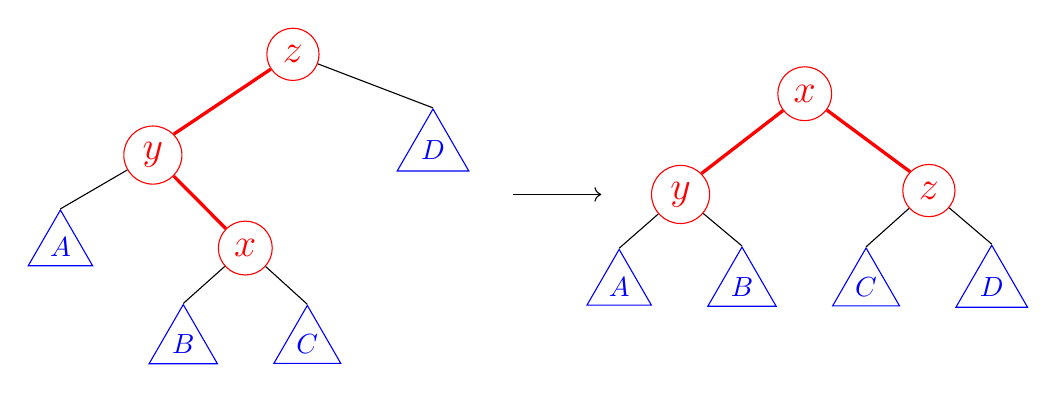
\begin{tikzpicture}[level distance = 35pt, sibling distance = 20pt,
  edge from parent/.style = {
    draw, edge from parent path = {(\tikzparentnode) -- (\tikzchildnode.north)}},
  ie/.style = {red, very thick, edge from parent path = {(\tikzparentnode) -- (\tikzchildnode.#1)}} % ie: internal edges
  ]

  \tikzset{every internal node/.style = {draw, circle, red, font = \Large}}
  \tikzset{every leaf node/.style = {draw, blue, regular polygon, regular polygon sides = 3, inner sep = 1pt}}

  \Tree [.$z$ 
	  \edge [ie = 45]; 
	  [.$y$
	    $A$
	    \edge [ie = 135]; 
	    [.$x$
	      $B$
	      $C$
	    ]
	  ] 
	  \node (d) {$D$};
	]

  \begin{scope}[xshift = 6.5cm, yshift = -0.50cm]
    \Tree [.$x$ 
	    \edge [ie = 45];
	    [.\node (y) {$y$};
	      $A$
	      $B$
	    ]
	    \edge [ie = 135]; 
	    [.$z$
	      $C$
	      $D$
	    ]
	  ]
  \end{scope}

  \draw[-<, shorten >= 40pt, shorten <= 50pt] (y) to ++(-2.5cm, 0);
\end{tikzpicture}
\end{document}
